\graphicspath{{chapters/images/}}
\chapter{T-COFFEE - ELISA}
T-COFFEE method is broadly based on the popular progressive approach to multiple alignment but avoids the most serious pitfalls caused by the greedy nature of this algorithm.
By pre-processing a data set of all pair-wise alignments between the sequences, a library is built to guide the progressive alignment.
Intermediate alignments are then based not only on the sequences to be aligned next, but also on how all of the sequences align with each other. This alignment information can be derived from heterogeneous sources such as a mixture of alignment programs and/or structure superposition.

\section{Introduction}
The most commonly used heuristic methods are based on the progressive-alignment strategy, with ClustalW being the most widely used implementation.
Although successful in a wide variety of cases, this method suffers from its greediness, as errors made in the first alignments cannot be rectified later as the rest of the sequences are added in.
T-Coffee is an attempt to minimize that effect, and although being still a greedy progressive method, it allows for much better use of information in the early stages.
\\
\\
\noindent
The main alternative to progressive alignment is the simultaneous alignment of all the sequences. Two such packages exist (MSA and DCA), based on the Carrilo and Lipman algorithm, but they remain an extremely CPU and memory-intensive approach.
Iterative strategies do not provide any guarantees about finding optimal solutions but are reasonably robust and much less sensitive to the number of sequences than their deterministic counterparts.
Alternatively, one might wish to consider local similarity, as occurs when two proteins share only a domain or motif.
Lalign, a variant of SW algorithm from the FASTA package, produces sets of non-overlapping local alignments from the comparison of two sequences.
For multiple sequences, the Gibbs sampler and Dialign2 are the main automatic methods, which perform well when there is a clear block of ungapped alignment shared by all of the sequences.
They perform poorly, however, on general sets of test cases when compared with global methods.
T-Coffee is aimed at providing a simple,  flexible and, most importantly, accurate solution to the problem of how to combine global and local multiple alignments.

\section{T-Coffee Algorithm}
T-Coffee (Tree-based Consistency Objective Function for alignment Evaluation) has two main features. First, it provides a simple and flexible means of generating multiple alignments, using heterogeneous data sources. The data from these sources are provided to T-Coffee via a library of pair-wise alignments.
The second main feature is the optimization method, which is used to find the multiple alignment that best fits the pair-wise alignments in the input library. We use a so-called progressive strategy, which is similar to that used in ClustalW. T- Coffee is a progressive alignment with an ability to consider information from all of the sequences during each alignment step, not just those being aligned at that stage. The progressive alignment is speed and simple, and a lower tendency to make errors is observed.
An overall scheme of T-Coffee algorithm is reported in figure \ref{fig:tcoffee}.

\begin{figure}[ht]
		\centering
		
\includegraphics[width=0.5\textwidth]{tcoffee}
		\caption{\label{fig:tcoffee}}
	\end{figure}

\subsection{Generating a primary library of alignments}
The primary library contains a set of pair-wise alignments between all of the sequences to be aligned.
In the library, we include information on each of the $N(N - 1)/2$ sequence pairs, where $N$ is the number of sequences.
\begin{itemize}
\item global alignments are computed with ClustalW
\item  local alignments are the ten top- scoring non-intersecting local alignments, between each pair of sequences, gathered using the Lalign
\end{itemize}
In the library, each alignment is represented as a list of pair-wise residue matches (e.g. residue x of sequence A is aligned with residue y of sequence B). In effect, each of these pairs is a constraint. All of these constraints are not equally important, some may come from parts of alignments that are more likely to be correct. We take this into account when computing the multiple alignment and give priority to the most reliable residue pairs by using a weighting scheme.

\subsection{Derivation of the primary library weights}
T-Coffee assigns a weight to each pair of aligned residues in the library. An ideal primary weight will reflect the correctness of a constraint. Sequence identity is used, as it is known to be a reasonable indicator of accuracy when aligning sequences with more than 30\% identity. This weighting scheme proved to be highly effective for a previous consistency-based objective function and has the advantage of great simplicity.
Each constraint receives a weight equal to percent identity within the pair-wise alignment it comes from.

\subsection{Combination of the libraries}
ClustalW and Laling primary libraries are pooled in a simple process of addition.
If any pair is duplicated between the two libraries, it is merged into a single entry that has a weight equal to the sum of the two weights. Otherwise, a new entry is created for the pair being considered.
Pairs of residues that did not occur are not represented (by default they will be considered to have a weight of zero).
This primary library can be used directly to compute a multiple sequence alignment.
For each pair of aligned residues in the library, we can assign a weight that reflects the degree to which those residues align consistently with residues from all the other sequences.

\subsection{Extending the library}
Fitting a set of weighted constraints into a multiple alignment is a well-known problem, formulated as an instance of the "maximum weight trace", an NP-complete problem. The genetic algorithm is robust but may require prohibitive computation time, while the graph-theory-based algorithm has a complexity only partially characterized and may fail in some cases for reasons that are difficult to predict.
The overall idea of the heuristic library extension algorithm is to combine information in such a manner that the final weight, for any pair of residues, reflects some of the information contained in the whole library. To do so, a triplet approach is used: the weight associated with a pair of residues will be the sum of all the weights gathered through the examination of all the triplets involving that pair.
The more intermediate sequences supporting the alignment of that pair, the higher its weight.
Extension will be carried out on each pair of residues of A and B. Once the operation is complete, sequence pair A and B will have gathered information from all the other sequences in the set.  The complete set of pairs constitutes the extended library.
The worst-case complexity of this computation is $O(N^3L^2)$ with L being the average sequence length. However, this will only occur when all the included pair-wise alignments are totally inconsistent. In practice the complexity is close to $(O)N^3L$.

\subsection{Progressive alignment strategy}
This alignment uses the weights in the extended library above to align the residues in the two sequences. This pair of sequences is then fixed and any gaps that have been introduced cannot be shifted later. Then the next closest two sequences are aligned or a sequence is added to the existing alignment of the first two sequences, depending which is suggested by the guide tree. The next two closest sequences or pre-aligned group of sequences are always joined.,until all the sequences have been aligned.
To align two groups of pre-aligned sequences the scores from the extended library are used, as before, but the average library scores in each column of existing alignment are taken.
The procedure does not require any additional parameters such as gap penalties, as the substitution values (the library weights) were computed on alignments where such penalties had already been applied.  Furthermore, high scoring segments that show consistency within the data set see their score enhanced by the extension to such a point that they become insensitive to gap penalties. In practice, this means that during the progressive phase, we use a dynamic-programming algorithm with gap-opening penalties and gap- extension penalties set to zero for aligning two sequences or two groups of pre-aligned sequences.

\section{Discussion}
T-Coffee is a new progressive method for sequence alignment. It can combine signals from heterogeneous sources (e.g. sequence-alignment programs, structure alignments, threading, manual alignment, motifs and specific constraints) into a unique consensus multiple sequence alignment.
The combination of local and global alignments leads to a significant increase in alignment accuracy.
The main difference from traditional progressive alignment methods is that, instead of using a substitution matrix for aligning the sequences, a position-specific scoring scheme is used (the extended library). Errors are less likely to occur during early stages of the progressive alignment. As a consequence, even though the paradigm "once a gap always a gap" remains true, misplacing gaps becomes much less likely.
The second important feature of T-Coffee is the combination of local and global information. The end-user benefits from the simplicity of the method and does not need to provide any extra parameter values.
\\
\\
\noindent
A key ingredient of the method is the primary weighting scheme.  The main reason why T-Coffee can tolerate small segments with high similarity is more likely to occur by chance is because short high-scoring segments are rarely consistent enough to have a strong effect on the position-specific scoring scheme after extension.
Moreover, final alignments are processed using dynamic programming,making it less likely for misplaced high-scoring segments to affect the alignment.
Although the protocol proposed here employs a minimal combination of local and global information, there is no theoretical limit to the number of methods that can be used. For instance, alignments from structural comparisons could be combined with sequence alignments. It is also possible to incorporate, in the library, information extracted from multiple alignments.


\graphicspath{{chapters/11/}}
\chapter{T-COFFEE - ILARIA}
\emph{T-Coffee: A Novel Method for Fast and Accurate Multiple Sequence Alignment}
We describe a new method (T-Coffee) for multiple sequence alignment that provides a dramatic improvement in accuracy with a modest sacrifice in speed as compared to the most commonly used alternatives.
\section{Introduction}
The simultaneous alignment of three or more nucleotide or amino acid sequences is one of the commonest tasks in bioinformatics.
Multiple alignments are an essential prerequisite to many analyses of protein families such as homology modeling or phylogenetic reconstruction, or to illustrate conserved and variable sites within a family.

\subsection{Reasons for the development}
\subsubsection{Once a gap, always a gap}
The most commonly used heuristic methods are based on the \textbf{progressive alignment strategy}, with \textbf{ClustalW} being the most widely used implementation.
The idea is to take an initial, approximate, phylogenetic tree between the sequences and to gradually build up the alignment, following the order in the tree. Although successful, this method suffers from its greediness.
Errors made in the first alignments cannot be rectified later as the rest of the sequences are added in.
Even though the paradigm ``once a gap always a gap'' remains true, misplacing gaps becomes much less likely.

\subsubsection{Global and local alignment}
Some methods attempt to carry out global alignments, where one tries to align the full lengths of the sequences with each other. Alternatively, one might wish to consider local similarity, as occurs when two proteins share only a domain or motif (Smith-Waterman, Lalign).
In principle, a method able to combine the best properties of global and local multiple alignments might be very powerful.
This is the second motivation for T-Coffee: the design of a method that provides a simple, flexible and, most importantly, accurate solution to the problem of how to combine information of this sort.

\begin{figure}[H]
\centering
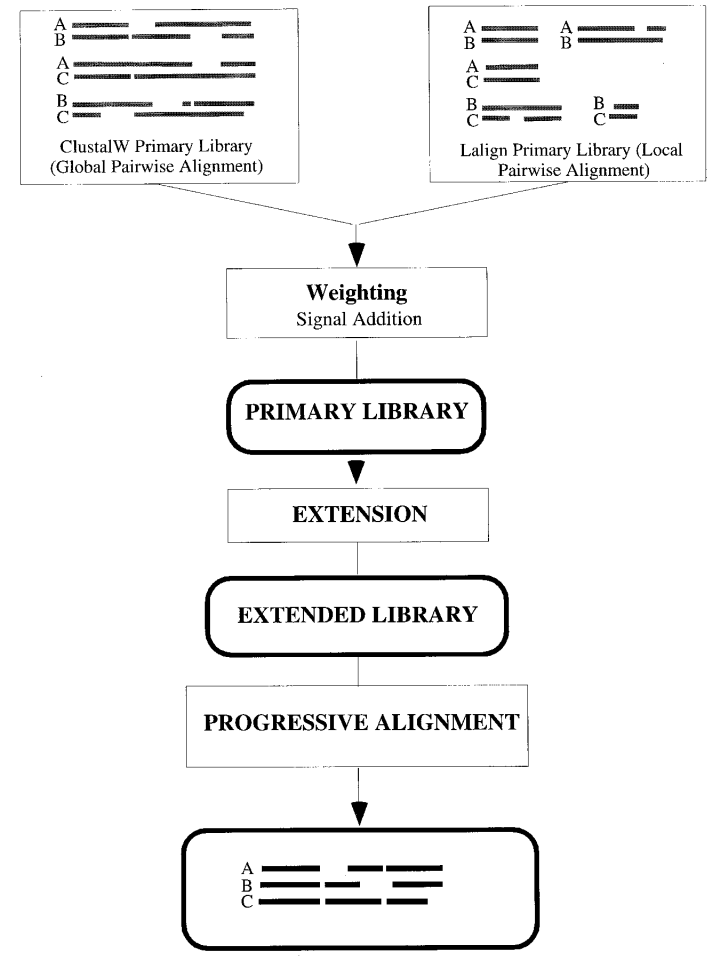
\includegraphics[width=0.5\linewidth]{1.png}
\caption{Layout of the T-Coffee strategy; the main steps required to compute a multiple sequence alignment using the T-Coffee method. Square blocks designate procedures while rounded blocks indicate data structures.}
\label{fig:structure}
\end{figure}

\section{T-Coffee Algorithm}
T-Coffee (Tree-based Consistency Objective Function for alignment Evaluation) has two main features.
\\
First, it provides a simple and flexible means of generating multiple alignments, using heterogeneous data sources. The data from these sources are provided to T-Coffee via a \textbf{library} of pair-wise alignments.
\\
The main feature of T-Coffee is the \textbf{optimization} method, which is used to find the multiple alignment that best fits the pair-wise alignments in the input library.
A so-called \textbf{progressive strategy} is implemented, which is similar to that used in ClustalW. The difference from CustalW is that T-Coffe makes use of the information in the library to carry out progressive alignment in a manner that allows us to consider the alignments between all the pairs while we carry out each step of the progressive multiple alignment.
This gives us progressive alignment, with all its advantages of speed and simplicity, but with a far lesser tendency to make errors like the one shown in Figure \ref{fig:2}(a), i.e. misalignment of the word CAT.
T-Coffee is a progressive alignment with an ability to consider information from all of the sequences during each alignment step, not just those being aligned at that stage.

\begin{figure}[H]
\centering
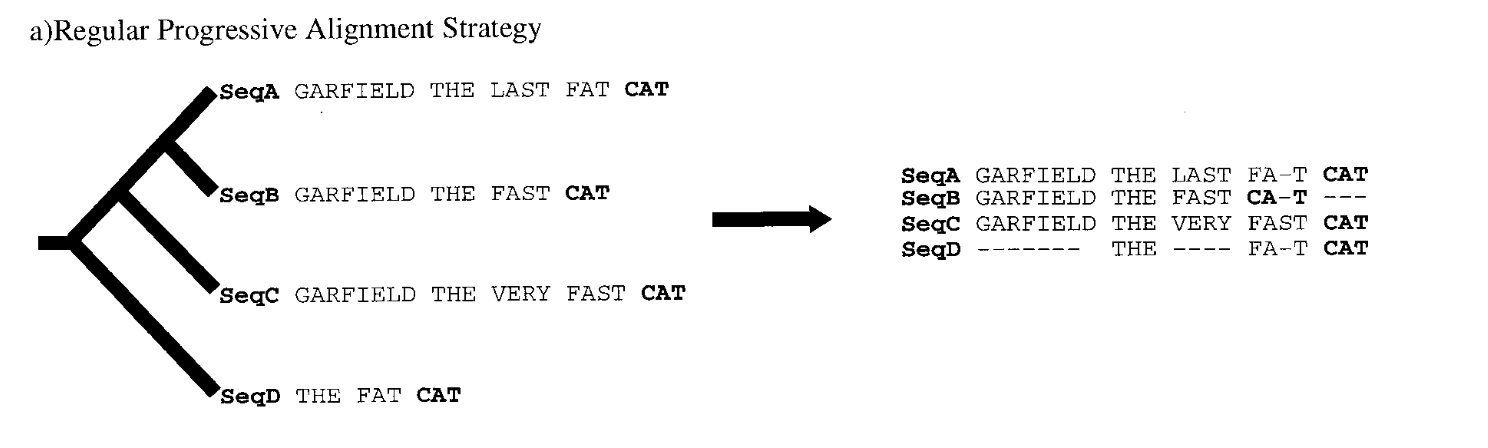
\includegraphics[width=0.8\linewidth]{2a.png}
c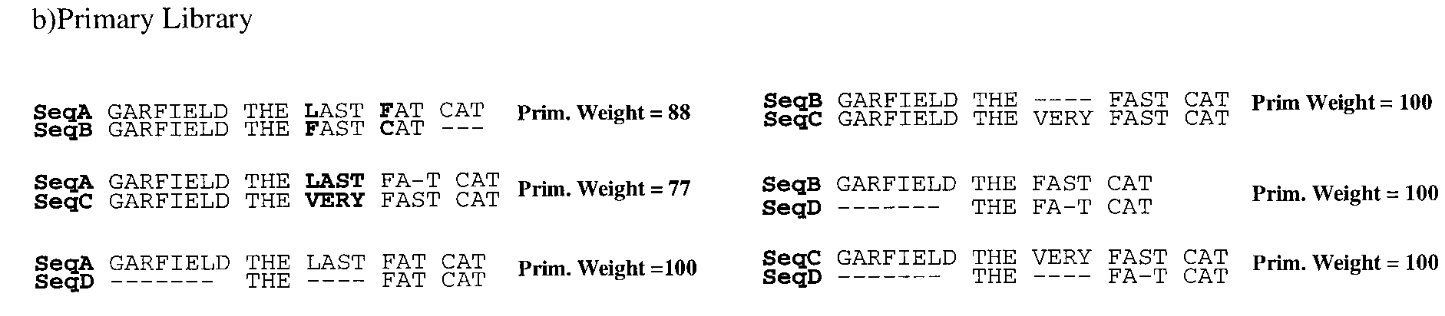
\includegraphics[width=0.8\linewidth]{2b.png}
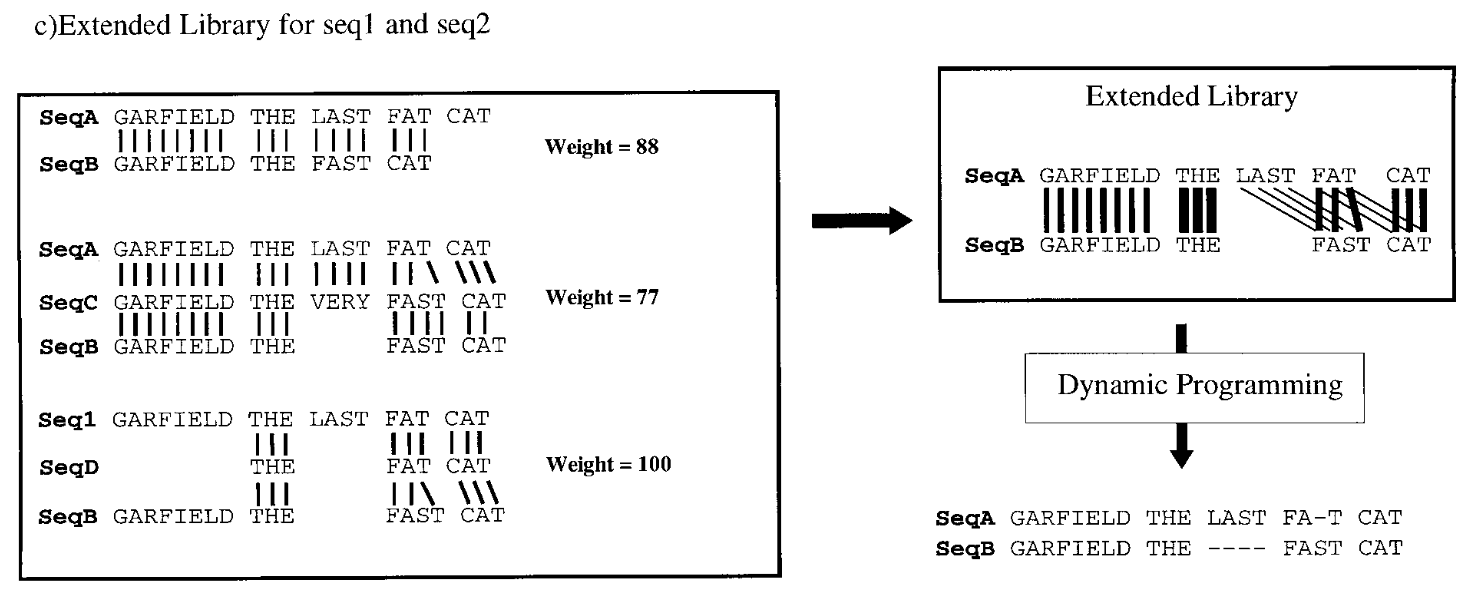
\includegraphics[width=0.8\linewidth]{2c.png}
\caption{The library extension. \textbf{(a) Progressive alignment}. Four sequences have been designed. The tree indicates the order in which the sequences are aligned when using a progressive method such as ClustalW. The resulting alignment is shown, with the word CAT misaligned. \textbf{(b) Primary library}. Each pair of sequences is aligned using ClustalW. In these alignments, each pair of aligned residues is associated with a weight equal to the average identity among matched residues within the complete alignment (mismatches are indicated in bold type). \textbf{(c) Library extension for a pair of sequences}. The three possible alignments of sequence A and B are shown (A and B, A and B through C, A and B through D). These alignments are combined, as explained in the text, to produce the position-specific library. This library is resolved by dynamic programming to give the correct alignment. The thickness of the lines indicates the strength of the weight.}
\label{fig:2}
\end{figure}


\subsection{Generating a primary library of alignments}
The primary library contains a set of pair-wise alignments between all of the sequences to be aligned.
In the library, we include information on each of the $N(N - 1)/2$ sequence pairs, where $N$ is the number of sequences. Here, we use two alignment sources for each pair of sequences, one \textbf{local} and one \textbf{global}.
The global alignments (Figures \ref{fig:structure} and \ref{fig:2}(b)) are constructed using ClustalW on the sequences, two at a time. The local alignments (Figure \ref{fig:structure}) are the ten top scoring non-intersecting local alignments, between each pair of sequences, gathered using the Lalign program.
\\
In the library, each alignment is represented as a list of pair-wise residue matches (e.g. residue x of sequence A is aligned with residue y of sequence B).
In effect, each of these pairs is a constraint.
All of these constraints are not equally important. Some may come from parts of alignments that are more likely to be correct. This is taken into account when computing the multiple alignment and give priority to the most reliable residue pairs. This is achieved by using a weighting scheme, which is described in subsection \ref{sub:weights}.

\subsection{Derivation of the primary library weights} \label{sub:weights}
T-Coffee assigns a weight to each pair of aligned residues in the library (Figure 2(b)).
The \textbf{sequence identity} weighting scheme is used, which has been prove to be effective and of great simplicity.
Libraries are lists of weighted pair-wise constraints. Each constraint receives a weight equal to percent identity within the pair-wise alignment it comes from (Figure \ref{fig:2}(b)).
For each set of sequences, two primary libraries are computed along with their weights, one using ClustalW (global alignments; Figure \ref{fig:2}(b)) and the second using Lalign (local).

\subsection{Combination of the libraries}
The aim is the efficient combination of local and global alignment information.
This is achieved by pooling the global and local primary libraries in a simple process of \textbf{addition}.
If any pair is duplicated between the two libraries, it is merged into a single entry that has a weight equal to the sum of the two weights.
Otherwise, a new entry is created for the pair being considered (process called unofficially "\textbf{stacking" of the signal}).
Pairs of residues that did not occur are not represented (weight of zero).
\\
This primary library can be used directly to compute a multiple sequence alignment.
However, we enormously increase the value of the information in the library by examining the consistency of each pair of residues with residue pairs from all of the other alignments.
For each pair of aligned residues in the library, we can assign a weight that reflects the degree to which those residues align consistently with residues from all the other sequences.
This process is called library extension (subsection \ref{sub:extension}).

\subsection{Extending the library} \label{sub:extension}
Fitting a set of weighted constraints into a multiple alignment is a well known NP-complete problem.
\\
We circumvent the problem by using a heuristic algorithm that we call \textbf{library extension} (Figure \ref{fig:2}(c)). The idea is to combine information in such a manner that the final weight, for any pair of residues, reflects some of the information contained in the whole library. To do so, a \textbf{triplet approach} is used, as summarized in Figure \ref{fig:2}(c).
\\
It is based on taking each aligned residue pair from the library and checking the alignment of the two residues with residues from the remaining sequences.
\subsubsection{A quick example}
For instance, let us consider the four sequences A, B, C
and D of Figure 2. Let us call A(G) the G of GARFIELD in sequence A, B(G) the equivalent G in sequence B and W(A(G), B(G)) the weight associated with this pair of symbols in the primary library. In the direct alignment of A and B, A(G) and B(G) are matched (Figure \ref{fig:2}(b) and (c)). Therefore, the initial weight for that pair of residues can be set to 88 (primary weight of the alignment of sequence A and B, which is the percent of identity of this pair). If we now look at the alignment of sequence A and sequence B through sequence C (Figure \ref{fig:2}(c)), we can see that the A(G) and C(G) are aligned, as well as C(G) and A(G). We conclude that there is an alignment of A(G) with B(G) through sequence C. We associate that alignment with a weight equal to the minimum of $W_1 = W(A(G), C(G))$ and $W_2 = W(C(G), B(G))$. Since $W_1 = 77$ and $W_2 = 100$, the resulting weight is set to 77. In the extended library, this new value is added to the previous one to give a total weight of 165 for the pair A(G), B(G). The complete extension will require an examination of all the remaining triplets. Not all of them bring information. For instance, the alignment of A and B through sequence D does not contain any information relative to A(G) or B(G), and, therefore, it has no influence on the weight associated with A(G) and B(G). In summary, the weight associated with a pair of residues will be the sum of all the weights gathered through the examination of all the triplets involving that pair.

\subsubsection{Alignment}
Weights will be zero for any residue pairs that never occur (this will be true of the majority of residue pairs). Otherwise, the weight will reflect a
combination of the similarity of the pair of sequences or sequence segments that the residue pair comes from and the consistency of that residue pair with all other residue pairs in the primary library. These scores can then be used to align any two sequences from our data set using conventional dynamic programming.
When one normally aligns a pair of sequences, one uses a set of scores derived from some general table of amino acid weights such as a Blosum matrix. In our case, we can replace that matrix with a set of scores that are specific to every possible pair of residues in our two sequences.
This will allow an alignment to be carried out that will take account of the particular residues in the two sequences but will also be guided towards consistency with all of the other sequences in the data set.

\subsection{Progressive alignment strategy}
The \textit{normal} progressive alignment strategy consists in creating a guide tree (a phylogenetic tree) using the neighbor-joining method.
The closest two sequences on the tree are aligned first using normal dynamic programming.
This pair of sequences is then fixed and any gaps that have been introduced cannot be shifted later. Then the next closest two sequences are aligned or a sequence is added to the existing alignment of the first two sequences, depending which is suggested by the guide tree.

As used here, the procedure does not require any additional parameters such as gap penalties. This stems, in part, from the fact that the substitution values (the library weights) were computed on alignments where such penalties had already been applied. Furthermore, high scoring segments that show consistency within the data set see their score enhanced by the extension to such a point that they become insensitive to gap penalties.

\section{Biological validation}
\textit{I chose not to report the comparisons with other tools and the complexity of the algorithm. If needed, exhaustive tabled can be found in the paper.}

\subsection{Application to serine/threonine kinases}
A major application of any alignment algorithm will be the delineation of motifs or domains.
19 sequences from a sub-family of the serine/threonine kinases were provided. Each sequence in the alignment contains a nucleotide-binding site (NBS).
In all these sequences, the NBS is followed by a second conserved motif toward the C terminus.
T-Coffee was able to accurately align 18 of the 19 NBSs, ClustalW was only able to correctly align 16 of these NBSs. The second motif is more difficult
because of the long indel in st11 yeast. Here as well, T-Coffee can properly align 18 of the motifs, while ClustalW get 15 correct.
As a result of combining local and global alignment information, T-Coffee managed to align almost all of the motifs as in the BaliBase reference alignment. Moreover, T-Coffee was the only program that correctly aligned the second motif of kp68 human, which is an interferon-induced kinase.
